% !TEX program = pdflatex
% ---------------------------------------------------------------------------
% simulator_figures.tex -- the tree-simulation layer: figures and equations.
%
% Build: LaTeX Workshop picks up the magic comment above (pdflatex; no latexmk
% on iris).  Ctrl+Alt+B builds, Ctrl+Alt+V opens the PDF beside the source.
% Or from a shell in this directory:  pdflatex simulator_figures.tex  (twice,
% for the cross-references).
%
% Figures are read from ../figures/ WITHOUT an extension, so pdflatex takes the
% vector .pdf when it exists and the .png otherwise.  Regenerate them with
%   scripts/submit.sh --mem 4G --time 0:30:00 --cpus 1 --part cpushort \
%       analyses/2026-09_simulator/src/10_fig_method.py
% Every number quoted in the S1 captions is in ../results/figS1_numbers.json.
%
% Notation follows the house register (sciphy_notes.md, H.6.0): lambda is the
% EDITING rate and f is reserved for functions, so neither appears here.
% ---------------------------------------------------------------------------
\documentclass[11pt]{article}
\usepackage[margin=1in]{geometry}
\usepackage{amsmath,amssymb,mathtools}
\usepackage{graphicx}
\usepackage{booktabs}
\usepackage{caption}
\usepackage{subcaption}
\usepackage[hidelinks]{hyperref}

\graphicspath{{../figures/}}
\captionsetup{font=small,labelfont=bf}

% house-register shorthands -- edit here and every equation follows
\newcommand{\bdrate}{b}          % birth (division) rate
\newcommand{\dthrate}{\delta}    % death rate
\newcommand{\turn}{\theta}       % turnover
\newcommand{\net}{r}             % net growth rate
\newcommand{\capt}{\rho}         % capture fraction
\newcommand{\E}{\mathbb{E}}
\newcommand{\Prob}{\mathbb{P}}
\DeclareMathOperator{\Binomial}{Binomial}
\DeclareMathOperator{\Exp}{Exp}

\title{The tree layer of the SciPhy/ENGRAM simulator:\\ figures and defining equations}
\author{Justin}  % edit
\date{Draft, \today}

\begin{document}
\maketitle

\noindent This document goes with the simulator in
\texttt{analyses/2026-09\_simulator/}, and has one section per figure. Section~\ref{sec:S1} covers the
\emph{tree layer} only: how a lineage tree is generated for one clone. Editing and dropout are
separate layers, added on top of these trees later, and are not described here.

% ===========================================================================
\section*{Notation}
% ===========================================================================

\begin{center}\small
\begin{tabular}{@{}lll@{}}
\toprule
symbol & meaning & units / range \\
\midrule
$n$ & cells captured from one clone & cells, $\ge 2$ \\
$T$ & time from the clone's founding cell to harvest & time; set to $1$ \\
$t$ & time since the founding cell, forward & $[0,T]$ \\
$\bdrate$ & per-cell division rate & $1/\text{time}$ \\
$\dthrate$ & per-cell death rate & $1/\text{time}$ \\
$\turn=\dthrate/\bdrate$ & turnover: deaths per division & $[0,1)$ \\
$\net=\bdrate-\dthrate$ & net growth rate & $1/\text{time}$ \\
$\capt$ & capture fraction: probability a cell alive at $T$ is sequenced & $(0,1]$ \\
$N(t)$ & cells alive at time $t$ (the whole clone, captured or not) & cells \\
$K$ & cells captured at harvest & cells \\
$\alpha,\beta$ & parameters of the law of $N(T)$, eq.~\eqref{eq:geom} & dimensionless \\
$\beta'$, $s$ & parameter of the law of $K$, and $s=\Prob(K\ge1)$, eq.~\eqref{eq:klaw} & dimensionless \\
$R$ & trees stored per library cell $(n,\capt,\turn)$ & $20$ \\
\bottomrule
\end{tabular}
\end{center}

% ===========================================================================
\section{Figure S1 --- how the simulator generates a tree}\label{sec:S1}
% ===========================================================================

\subsection{What is modelled, and what is taken from the data}

Each clone is simulated separately. It starts from one founding cell at $t=0$. Every cell
alive at time $t$ divides at rate $\bdrate$ and dies at rate $\dthrate$, independently of every
other cell and of its own history. At harvest, $t=T$, each surviving cell is captured
independently with probability $\capt$. The tree we would observe is the \emph{reconstructed
tree}: the genealogy of the captured cells only.

\paragraph{Clone size is conditioned on, not simulated.} One homogeneous birth--death process
has a geometric (exponentially bounded) size distribution, eq.~\eqref{eq:geom}. It cannot produce
Park's clone sizes. Fitted to each arm's median clone size, it predicts between
$2.8\times10^{-14}$ (Mouse3) and $10^{-119}$ or fewer (Mouse1, Mouse2) clones as large as the
largest observed one, and exactly one is observed in every arm (\texttt{sciphy\_notes.md}
\S S3.4). So we do not simulate how large a clone gets. We take each clone's captured size $n$
from the data and simulate the tree \emph{conditional on} $K=n$. Heterogeneity in growth rate
\emph{between} clones is then absorbed, and constant rates are assumed only \emph{within} a clone.

\subsection{The birth--death process}

Let $N(t)$ cells be alive. Each carries two exponential clocks, one for division (rate
$\bdrate$) and one for death (rate $\dthrate$). The simulator is an exact Gillespie loop over
events, with no time step. With $N$ cells alive, the total event rate is
\begin{equation}
  A(N) = N(\bdrate+\dthrate),
  \label{eq:propensity}
\end{equation}
and three facts define the whole process:
\begin{align}
  \Delta t &\sim \Exp\!\big(A(N)\big)
    && \text{time to the next event in the clone,} \label{eq:wait}\\
  \Prob(\text{division}) &= \frac{\bdrate}{\bdrate+\dthrate},
  \quad \Prob(\text{death}) = \frac{\dthrate}{\bdrate+\dthrate}
    && \text{independent of $\Delta t$,} \label{eq:type}\\
  \text{affected cell} &\sim \text{Uniform}\{1,\dots,N\}
    && \text{independent of both.} \label{eq:who}
\end{align}
A division replaces the cell with two daughters, and a death removes it. The loop stops at the
first event past $T$.

\subsection{Parameterisation}

Only two numbers matter for the size of the clone at harvest: the net rate $\net$ and the
turnover $\turn$. Given a target $(n,\capt,\turn)$, the simulator (\texttt{rate\_params} in
\texttt{01\_bdtree.py}) sets
\begin{equation}
  \net = \frac{\ln(n/\capt)}{T}, \qquad
  \bdrate = \frac{\net}{1-\turn}, \qquad
  \dthrate = \turn\,\bdrate,
  \label{eq:params}
\end{equation}
so that the expected clone size at harvest is the size needed to yield $n$ captured cells on
average:
\begin{equation}
  \E[N(T)] = e^{\net T} = \frac{n}{\capt}, \qquad \E[K] = \capt\,\E[N(T)] = n .
  \label{eq:mean}
\end{equation}
$T=1$ fixes the time unit, so every time in the figures is a fraction of the experiment. Note
that $\turn$ does not change $\E[N(T)]$: at a fixed target, raising the turnover raises
$\bdrate$ and $\dthrate$ together.

\emph{Caveat.} $T$ is a free scale only for the tree layer on its own. Once editing is added, $T$
is pinned by the measured editing depth $\Lambda=\lambda T$, where $\lambda$ is the editing rate.

\subsection{Size at harvest}

$N(T)$ has a classical closed form (Kendall). With $u=e^{\net T}$,
\begin{equation}
\begin{gathered}
  \alpha = \frac{\dthrate(u-1)}{\bdrate u-\dthrate},\qquad
  \beta  = \frac{\bdrate(u-1)}{\bdrate u-\dthrate},\\[2pt]
  \Prob(N(T)=0)=\alpha,\qquad
  \Prob(N(T)=m)=(1-\alpha)(1-\beta)\,\beta^{\,m-1}\quad (m\ge1).
\end{gathered}
  \label{eq:geom}
\end{equation}
$\alpha$ is the probability that the clone is extinct by $T$. For large $u$, $1-\alpha\to 1-\turn$:
at turnover $0.7$, most clones die out.

\subsection{Capture, and conditioning on clone size}

Each survivor is captured independently with probability $\capt$:
\begin{equation}
  K \mid N(T) \sim \Binomial\big(N(T),\,\capt\big),
  \qquad\text{captured set} \mid K \;\sim\; \text{uniform $K$-subset of the survivors.}
  \label{eq:capture}
\end{equation}
Thinning a geometric by a binomial leaves it geometric. Writing $c=1-\beta(1-\capt)$,
\begin{equation}
  \boxed{\;
  \Prob(K=k) = s\,(1-\beta')\,\beta'^{\,k-1}\quad (k\ge1),\qquad
  \beta'=\frac{\capt\beta}{c},\qquad
  s=\Prob(K\ge1)=\frac{(1-\alpha)\capt}{c}. \;}
  \label{eq:klaw}
\end{equation}
Given at least one captured cell, $K$ is geometric with parameter $\beta'$.

\paragraph{Conditioning by rejection.} An \emph{attempt} runs eqs.~\eqref{eq:wait}--\eqref{eq:capture}
from one founding cell. The attempt is accepted if and only if $K=n$ exactly (\texttt{tol}\,$=0$);
otherwise it is discarded and a fresh, independently seeded attempt starts. The accepted tree is
therefore an exact draw from the process conditioned on $K=n$. The acceptance probability is
$a(n)=\Prob(K=n)$ from eq.~\eqref{eq:klaw}. By eq.~\eqref{eq:mean}, $\E[K\mid K\ge1]=n/s$, so
\begin{equation}
  a(n) = \frac{s^2}{n}\Big(1-\frac{s}{n}\Big)^{n-1} \approx \frac{s^2 e^{-s}}{n},
  \qquad
  \E[\text{attempts per accepted tree}] = \frac{1}{a(n)} \approx \frac{n\,e^{s}}{s^2}.
  \label{eq:attempts}
\end{equation}

\paragraph{Why only the counts are simulated first.} By eq.~\eqref{eq:who}, which cell an event
hits is independent of when it happens and of what kind of event it is. The law therefore
factorises:
\begin{equation}
  \Prob(\text{genealogy}) = \Prob\big(\text{count path } N(\cdot)\big)\times
  \Prob\big(\text{which cell each event hits} \mid N(\cdot)\big).
  \label{eq:factor}
\end{equation}
The acceptance test reads only $N(T)$ and the binomial draw. So pass~1 simulates the count path
alone, vectorised and with no tree. Only an accepted attempt is replayed from the same seed, in
pass~2, which assigns events to cells and builds the genealogy. Both passes sample the same
distribution. The rejected attempts, about $1/a(n)$ of them, never allocate a node.

\subsection{The reconstructed tree}

Let $S$ be the $n$ captured cells, and let $\mathcal{A}$ be every node of the full genealogy that
has a captured descendant. Reconstruction:
\begin{enumerate}
  \item \textbf{delete} every node outside $\mathcal{A}$: dead lineages, and survivors that were
        not captured, together with any ancestry they do not share with $S$;
  \item \textbf{suppress degree-2 nodes}: a division in $\mathcal{A}$ where only one daughter has
        a captured descendant is invisible in the data, so its two branches are spliced into one.
\end{enumerate}
The result is a binary tree with $n$ tips at $t=T$, $n-1$ visible branch points and $2n-1$
nodes, plus a stem from the founding cell at $t=0$ down to the first visible branch point.

\paragraph{Why the reconstructed tree is not itself a birth--death tree.} Step 2 removes branch
points unevenly in time. Deep divisions are more likely to be spliced out than recent ones,
because a deep lineage has had longer for all but one of its sub-lineages to die or go
uncaptured. The law of the reconstructed tree given $n$ is known in closed form, and we use it only
to check the simulator: (i) the shape is uniform over ranked histories, so
$\Prob(\text{root splits } j:n-j)=1/(n-1)$ (Yule--Harding), whatever $\bdrate$, $\dthrate$ and
$\capt$ are; and (ii) the $n-1$ branching times, measured back from harvest as $x=T-t$, are iid
with CDF
\begin{equation}
  G(x) = \frac{h(x)-\capt}{h(T)-\capt},\qquad
  h(x) = \frac{\capt\,\net}{\bdrate\capt + \big(\bdrate(1-\capt)-\dthrate\big)e^{-\net x}} ,
  \label{eq:G}
\end{equation}
where $h(x)$ is the probability that a lineage alive at time $x$ before harvest leaves at least
one captured descendant. Together, (i) and (ii) mean that \emph{all} of $\bdrate$, $\dthrate$ and $\capt$ act
on the branching times and none on the shape. In practice the tree contributes about one
effective number: how deep the coalescences sit.

% ---------------------------------------------------------------------------
\begin{figure}[p]
  \centering
  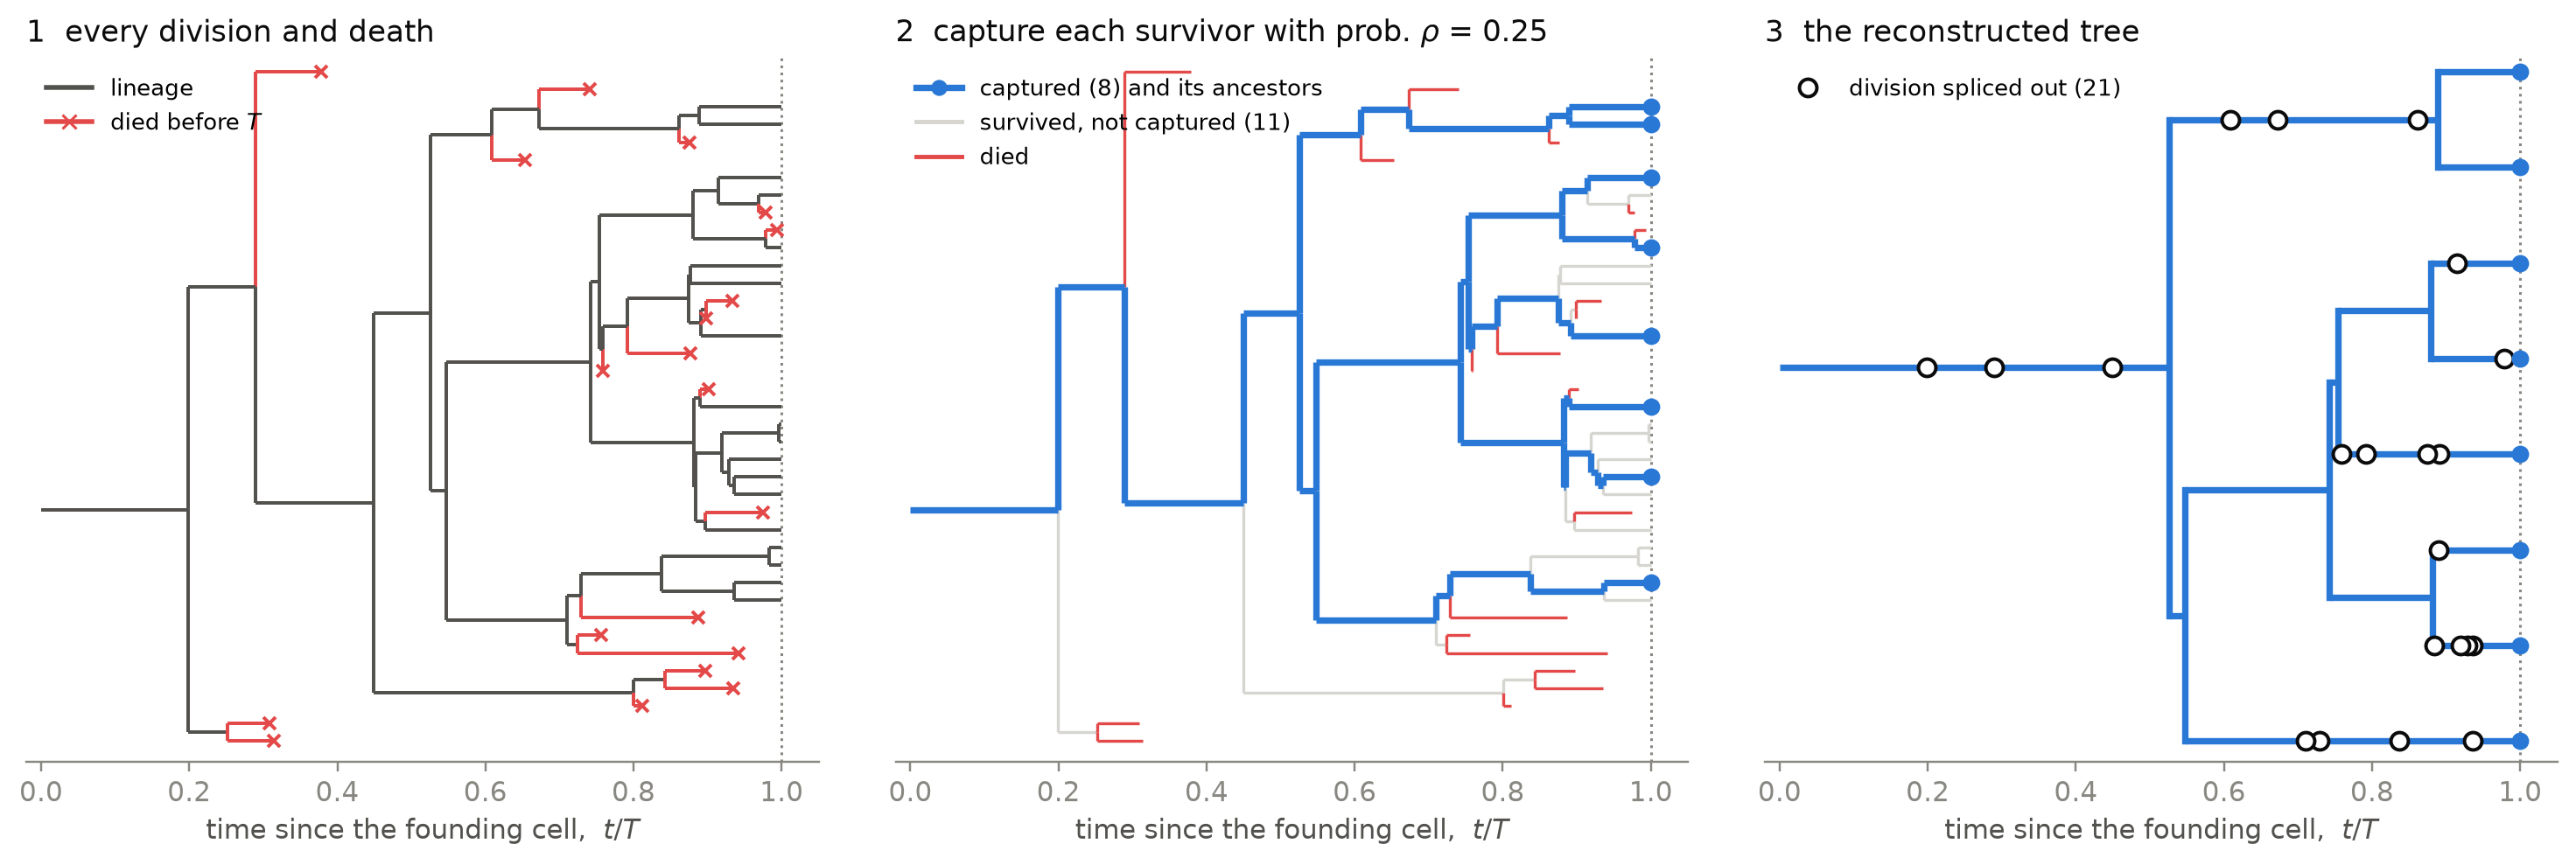
\includegraphics[width=\textwidth]{figS1a_forward}
  \caption{\textbf{One simulated tree, through the three stages of the simulator.}
  Clone target $n=8$ captured cells, capture fraction $\capt=0.25$, turnover $\turn=0.5$, which
  by eq.~\eqref{eq:params} gives $\bdrate=6.93$ and $\dthrate=3.47$ per unit $T$. The horizontal
  axis is time since the founding cell as a fraction of the experiment; vertical position only
  separates lineages.
  \textbf{(1)} The full process: 38 divisions and 20 deaths (red, $\times$), leaving 19 cells
  alive at harvest (dotted line).
  \textbf{(2)} Capture: each survivor is kept with probability $0.25$, independently. Here 8 of
  the 19 were captured (blue dots), and the attempt is accepted because $K=n$. Blue marks the
  captured cells and their ancestors; the 11 uncaptured survivors are grey.
  \textbf{(3)} The reconstructed tree: 8 tips, 7 visible branch points, 15 nodes. Each open
  circle is one of the 21 divisions where only one daughter left a captured descendant; it
  cannot be seen in the data, so it is spliced out. Of the 77 nodes in the full genealogy, 15
  survive. Three of the spliced divisions sit on the stem before $t=0.53$, so the clone's
  earliest visible branch point is about halfway through the experiment.
  \emph{Illustration choice:} this is the first accepted attempt whose full genealogy was small
  enough to draw ($\le120$ nodes; 160 attempts in). Capture follows the simulator's own rule,
  eq.~\eqref{eq:capture}. The reconstruction agrees exactly with the production code
  (\texttt{bd.reconstruct}).}
  \label{fig:S1a}
\end{figure}

\begin{figure}[p]
  \centering
  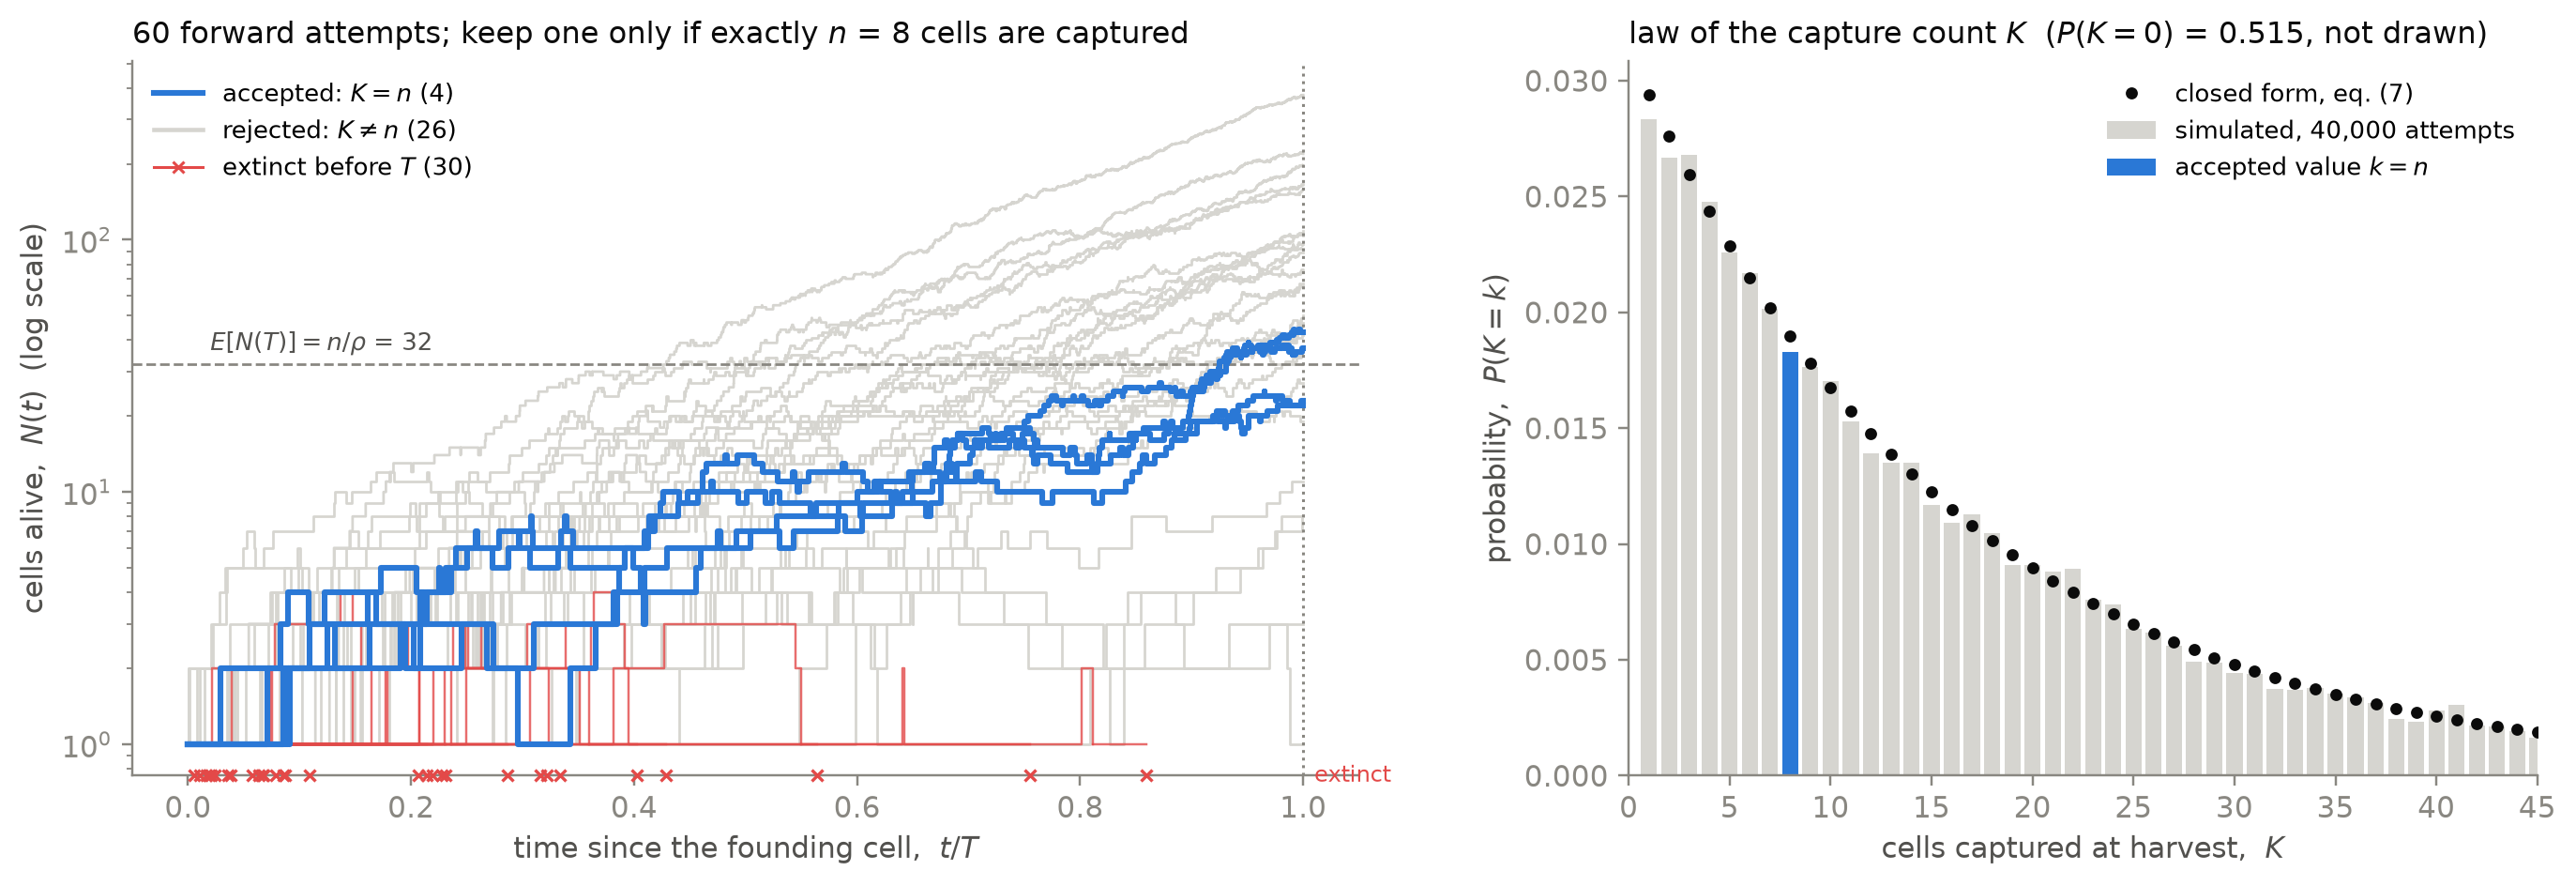
\includegraphics[width=\textwidth]{figS1b_condition}
  \caption{\textbf{Conditioning on the observed clone size.} Same parameters as
  Fig.~\ref{fig:S1a} ($n=8$, $\capt=0.25$, $\turn=0.5$).
  \textbf{Left:} 60 independent forward attempts, each showing the number of cells alive,
  $N(t)$, on a log scale. At harvest each attempt draws its capture count
  $K\sim\Binomial(N(T),0.25)$. The attempt is kept only if $K=8$ (blue, 4 of 60) and is
  otherwise discarded (grey, 26). Half the attempts (red, 30) go extinct before harvest, mostly early, while
  the clone is still only a few cells. The dashed line is the
  mean clone size the parameters target, $\E[N(T)]=n/\capt=32$ cells (eq.~\ref{eq:mean}).
  \textbf{Right:} the law of $K$. Grey bars are 40,000 simulated attempts; black dots are the
  closed form, eq.~\eqref{eq:klaw}. \emph{Reading rule:} if the simulator is right, the dots sit
  on the bars to within Monte Carlo noise. Across $k=1$--$59$ the largest deviation is 2.6
  standard errors, consistent with noise for 59 values. The blue bar is the only value
  accepted: $\Prob(K=8)=0.0190$ exact against $0.0183$ simulated. So one tree costs on average
  $1/a(n)=52.7$ attempts. $\Prob(K=0)=0.515$ ($0.518$ simulated) is off the axis.}
  \label{fig:S1b}
\end{figure}

\subsection{The tree library}

Simulated trees are generated once and stored, and every later sweep over editing and dropout
parameters \emph{re-decorates the same trees}, so those comparisons are paired. The library covers
the \emph{range} of clone sizes rather than Park's clone list: every integer $n$ from $2$ to $64$
(where 97.1\% of Park clones lie; median 8 cells), plus log-spaced sizes up to $11{,}081$ that
include each arm's largest clone exactly. A Park arm is rebuilt later by drawing, for each real
clone of size $n_C$, a stored tree at the nearest stocked size, so the arm's true size
\emph{distribution} is reproduced. Each stored tree keeps its parent array, branch lengths, seed
and accepting attempt index, and it replays bit-identically.

\begin{figure}[p]
  \centering
  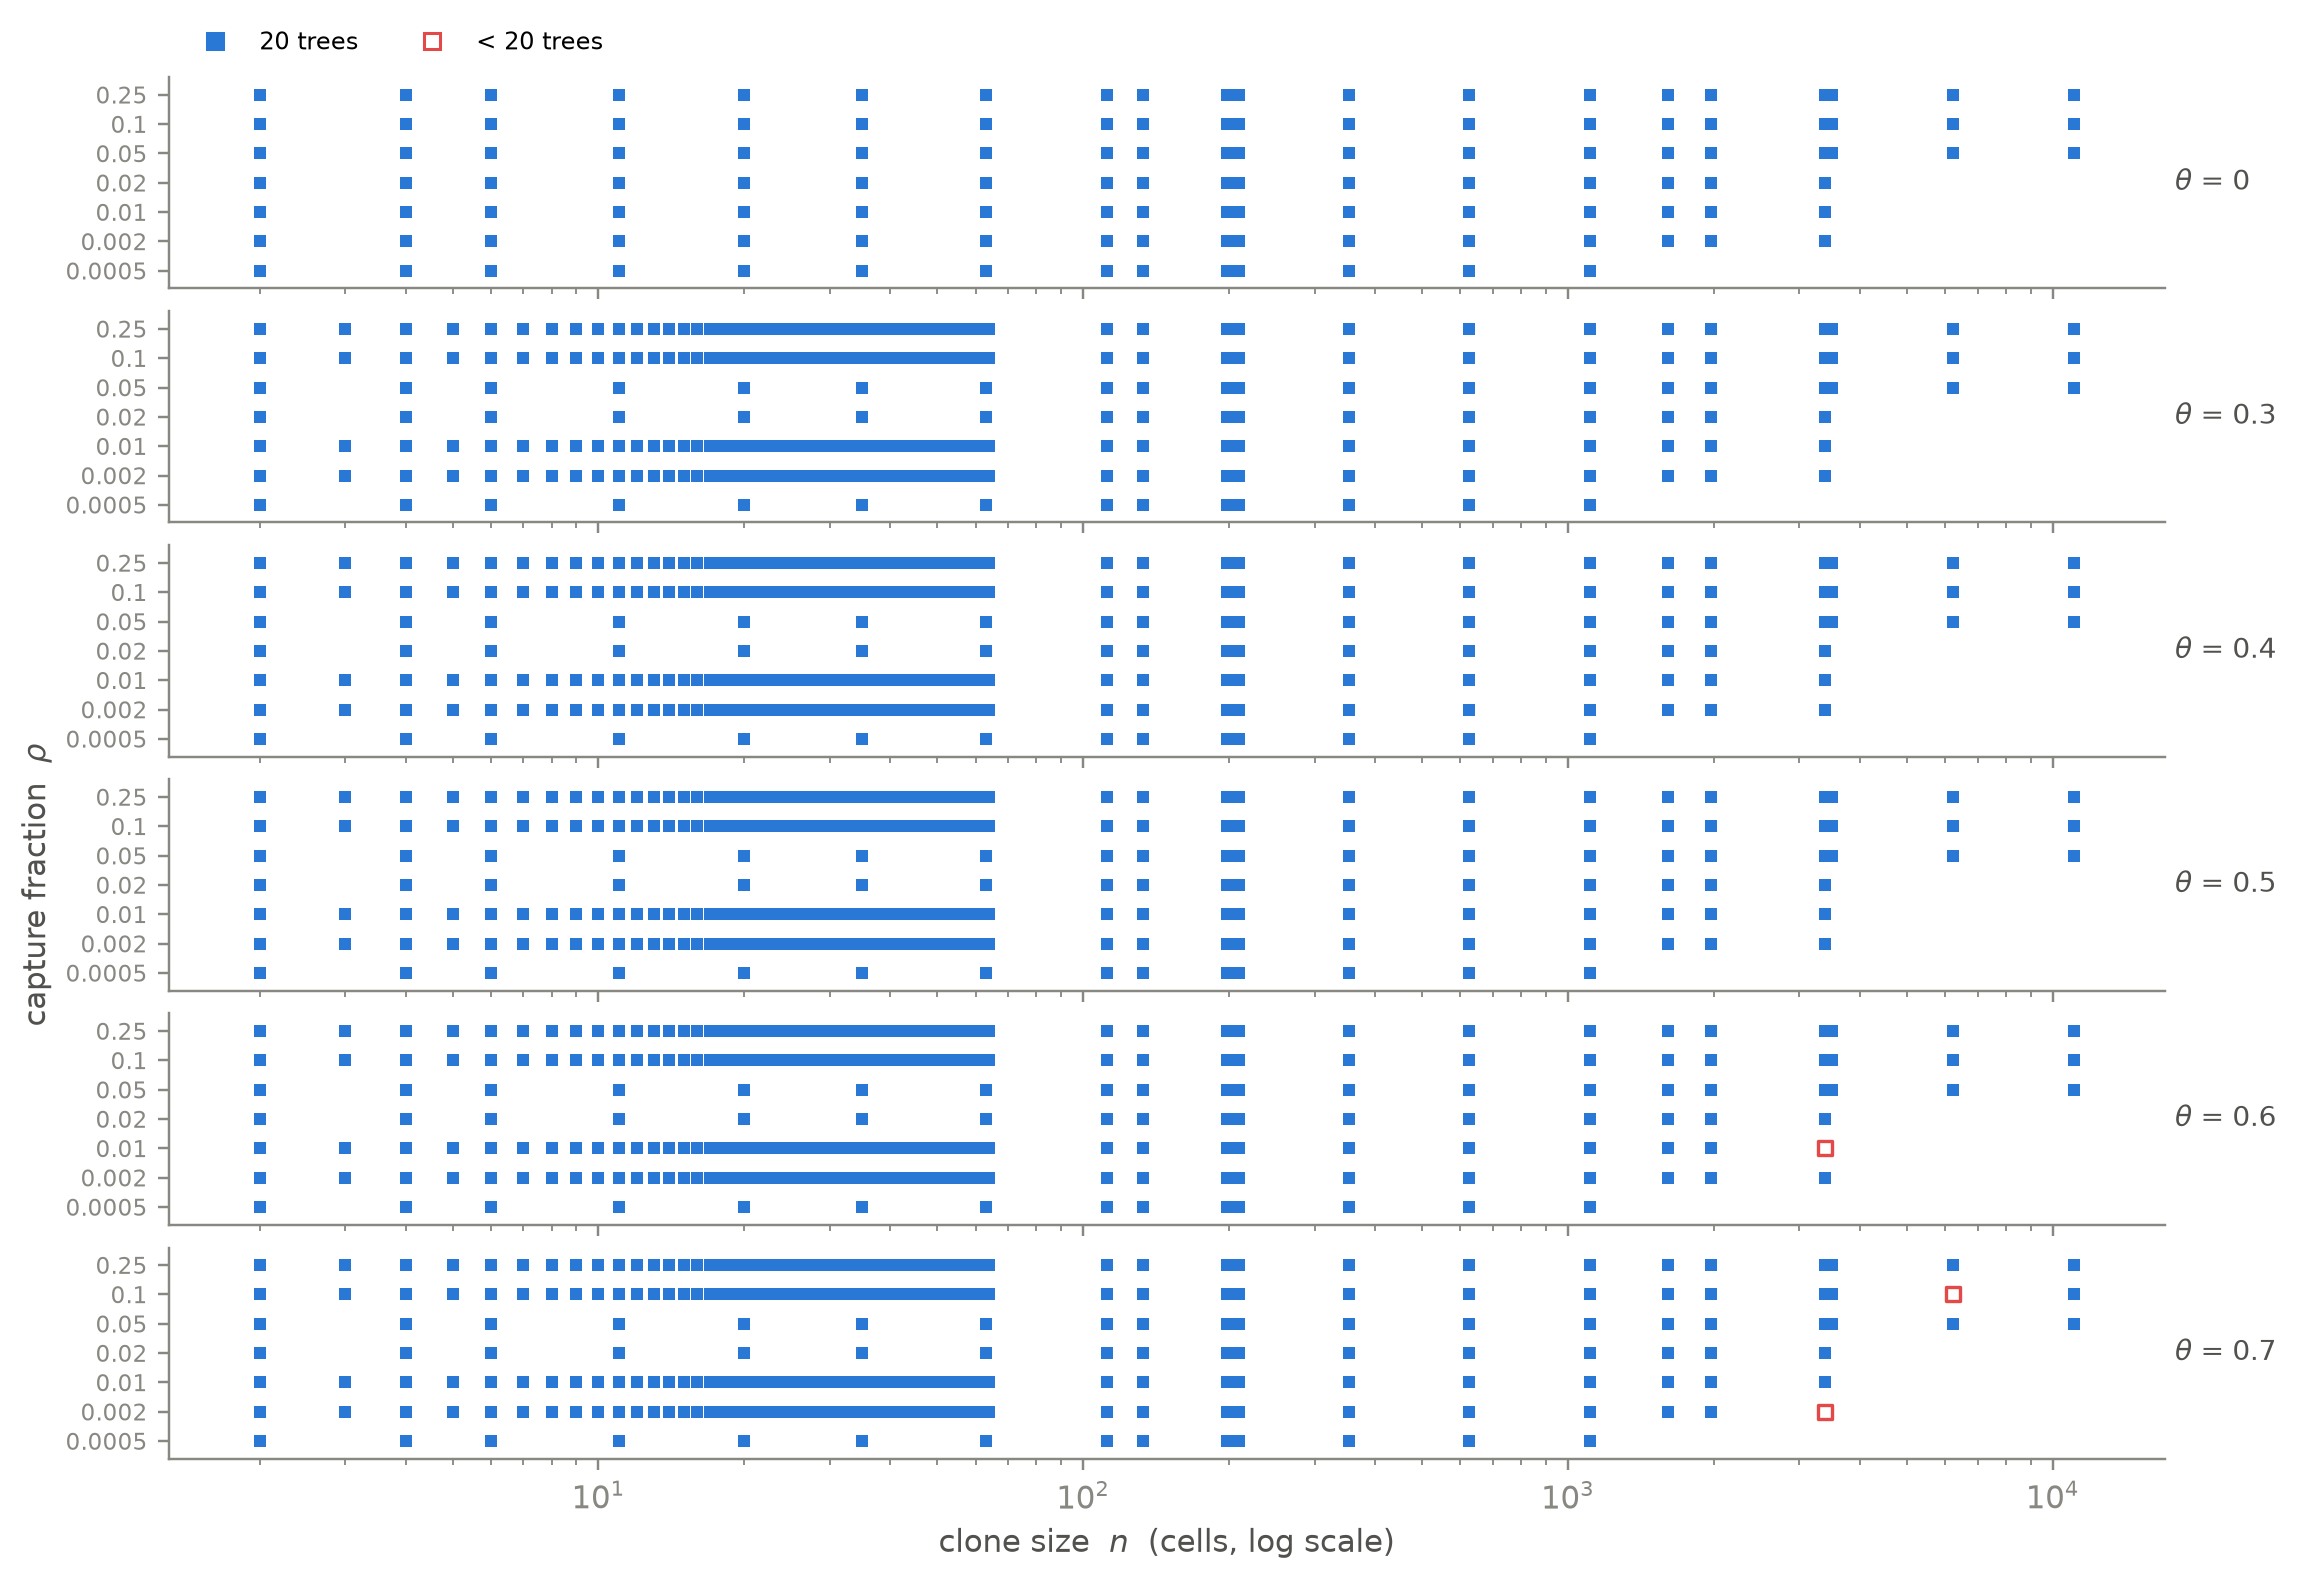
\includegraphics[width=\textwidth]{figS1c_library}
  \caption{\textbf{What the tree library holds.} One row of small multiples per turnover
  $\turn\in\{0,0.3,\dots,0.7\}$. Within a row, each square is one library cell: clone size $n$
  (horizontal, log scale) against capture fraction $\capt$ (vertical). Filled blue means the
  target $R=20$ trees are stored; open red means fewer. The dense band at $n\le64$ is the
  every-integer range, stocked at $\capt\in\{0.25,0.1,0.01,0.002\}$; the $\turn=0$ reference and
  the extended $\capt\in\{0.05,0.02,0.0005\}$ are stocked on the log-spaced sizes only. The mouse-like
  capture fractions stop at the mouse size range ($n\le3{,}387$; $n\le1{,}112$ at
  $\capt=0.0005$), because larger clones at those $\capt$ describe no arm that exists and cost
  $\propto n^2/\capt$.
  \emph{Complete library, 2026-09-23:} 1,870 cells and 37,380 trees, zero structure faults. The
  three open cells are known under-fills, all at high turnover: $(3387,0.002,0.7)$ 18,
  $(3387,0.01,0.6)$ 8 and $(6237,0.1,0.7)$ 14 trees.}
  \label{fig:S1c}
\end{figure}

% ===========================================================================
\section[Figure S2 --- validation]{Figure S2 --- validation: does the code simulate eqs.~(\ref{eq:propensity})--(\ref{eq:capture})?}\label{sec:S2}
% ===========================================================================

Section~\ref{sec:S1} defines a process. Validation (\texttt{02\_validate\_tree.py}) asks whether
the code produces it. Each check compares simulated trees with a property that is already known in
closed form and was verified independently in \texttt{sciphy\_notes.md} \S S3.3, so a failure points
to the code rather than the algebra. There are five checks:

\begin{center}\small
\begin{tabular}{@{}l p{0.19\textwidth} p{0.33\textwidth} p{0.3\textwidth}@{}}
\toprule
check & compares & closed form & what a failure would mean \\
\midrule
A & law of $N(T)$ & eq.~\eqref{eq:geom}, $\E[N(T)]=e^{\net T}$ & the Gillespie loop is wrong \\
B & tree structure & $n$ tips, $n-1$ branch points, 2 children each & pruning or splicing is wrong \\
C & root split & eq.~\eqref{eq:rootsplit} & pruning distorts the \emph{shape} \\
D & labelled histories & uniform over $n!(n-1)!/2^{n-1}$ & a subtler shape error that C misses \\
E & fast vs.\ naive code & each other, in distribution & the two-pass shortcut, eq.~\eqref{eq:factor}, is wrong \\
\bottomrule
\end{tabular}
\end{center}

\subsection{How a check is read}\label{sec:reading}

Most checks compare frequencies. A check has $m$ \emph{cells} (outcomes such as ``the smaller root
clade has $k$ tips''). Cell $j$ has expected probability $p_j$, and is observed $c_j$ times in $M$
simulated trees. Its deviation, in standard errors, is
\begin{equation}
  z_j = \frac{c_j/M - p_j}{\sqrt{p_j(1-p_j)/M}} ,
  \label{eq:z}
\end{equation}
which is approximately $\mathcal{N}(0,1)$ if the simulator is right. The check reports its
\emph{worst} cell, $Z_{\max}=\max_j |z_j|$.

\paragraph{The threshold has to grow with $m$.} The largest of $m$ noisy deviations is larger than a
typical one, even when nothing is wrong. So a flat ``flag above 3~se'' is wrong. For each check, the
critical value $z^{*}_{99}(m,M)$ is instead the 99th percentile of $Z_{\max}$ under the null. It is
computed by Monte Carlo: draw $40{,}000$ multinomial samples of size $M$ over $m$ equiprobable
cells, and take the 99th percentile of $Z_{\max}$ across them. At $M=4{,}000$ it is $2.56$ for
$m=2$, $3.03$ for $m=4$, $3.47$ for $m=18$ and $4.42$ for $m=180$. The flat rule once called a
correct run a \textsc{fail} at $3.14$ on a 180-cell check, whose statistic sat at the 62nd
percentile of its own null. The number actually reported is the ratio
\begin{equation}
  \text{score} = \frac{Z_{\max}}{z^{*}_{99}(m,M)} ,
  \qquad \text{pass if score} < 1 .
  \label{eq:score}
\end{equation}
\emph{Reading rule.} $1$ is the failure line. A correct simulator gives scores spread over roughly
$0.3$--$1$. One job runs about 15 checks, each at its own 99th percentile, so about 14\% of correct
runs will have one score above $1$. A single score near $1$ is therefore expected. A \emph{bug}
shows up as a score far above $1$ (the one real bug found scored 63~se; see below).

\subsection{\texorpdfstring{Check A: the law of $N(T)$}{Check A: the law of N(T)}}

Checks the Gillespie loop, eqs.~\eqref{eq:wait}--\eqref{eq:who}, against the geometric law,
eq.~\eqref{eq:geom}. Run $20{,}000$ attempts with no conditioning, and record $N(T)$ for each.
Compare the extinction fraction with $\alpha$, the sample mean with $e^{\net T}$, and
$\Prob(N(T)=m)$ with $(1-\alpha)(1-\beta)\beta^{m-1}$ at $m=1,2,3,5,8$. Run at $n=64$,
$\capt=0.5$ (so $\E[N(T)]=128$) and turnovers $0$, $0.3$ and $0.75$. Worst row: $1.91$~se.

\subsection{Checks C and D: the shape of the reconstructed tree}\label{sec:shape}

These are the most informative checks, because the prediction contains \emph{no parameters at
all}. Conditional on $n$ tips, the reconstructed tree of a constant-rate birth--death process is
uniform over \emph{ranked labelled histories}: the order in which pairs of lineages merge, going
back in time. That is true for any $\bdrate$, $\dthrate$ and $\capt$ (\S S3.3.3). Two consequences
are testable.

\paragraph{C --- root split.} Label the two clades below the root so that the smaller one has $k$
tips. Under a uniform ranked history, the left clade has each size $1,\dots,n-1$ with equal
probability $1/(n-1)$. Folding the two sides together gives
\begin{equation}
  \Prob(\text{smaller root clade has $k$ tips}) =
  \begin{cases}
    \dfrac{2}{n-1}, & 1 \le k < n/2,\\[6pt]
    \dfrac{1}{n-1}, & k = n/2 \ (\text{$n$ even}).
  \end{cases}
  \label{eq:rootsplit}
\end{equation}
At $n=8$ the four cells are $2/7, 2/7, 2/7, 1/7$.

\paragraph{D --- labelled histories.} This is the full version of C. At small $n$ the ranked
labelled histories can be enumerated: there are $n!(n-1)!/2^{n-1}$ of them, $18$ at $n=4$ and $180$
at $n=5$. Randomly permute the tip labels of each simulated tree, since the simulator's cell ids
carry creation order. Then every history should appear with frequency $1/18$ or $1/180$. D catches
distortions that happen to preserve the root split, such as a wrong joining rule deeper in the
tree. It cannot be run at $n=8$: there are 1,587,600 histories, far more than the trees available.

\paragraph{Why these two are the hard test of reconstruction.} Nothing in the prediction depends on
how much pruning a tree needed. The \emph{pruning load} is the number of full-genealogy nodes
traversed per visible branch point, $(|\mathcal{A}|-1)/(n-1)$. It ranged from $2.9$ ($\capt=0.5$,
$\turn=0$) to $65.2$ ($\capt=8\times10^{-4}$, $\turn=0.75$, $n=4$), a 22-fold span. If splicing ever
dropped or misattached a branch, eq.~\eqref{eq:rootsplit} would fail more badly as the load grew.
It held at every load.

\paragraph{The one real failure, and what it taught.} The first run \textsc{fail}ed C at $63$~se.
It passed D in the \emph{same} run. That is a contradiction, because the root split is a function
of the labelled history. So the fault had to be in the instrument, not the simulator. The function
counting tips below each node visited the nodes in id order, which is correct for the full
genealogy but inverted for the reconstructed tree, where a child has a \emph{smaller} id than its
parent. At $n=4$ the wrong computation happens to be right for both possible shapes, which is why
it survived the first look. Check E saw nothing, because both implementations it compares went
through the same broken counting function.

\subsection{Checks B and F: structure, at every size}

Every accepted tree must have exactly $n$ tips at $t=T$, $n-1$ branching times inside $(0,T)$,
$2n-1$ nodes, and exactly two children at every internal node. A missed splice leaves a node with
one child, and this is the only check that sees it directly. B runs on every tree used in C and D.
F repeats it at large $n$ ($210$, $1{,}024$ and $3{,}387$), where C and D have too many cells to
test, which closes the gap between ``validated at $n\le8$'' and ``used at $n\le11{,}081$''. The tree
library runs B on every one of its trees as it writes them.

\subsection{Check E: two independent implementations}

\texttt{simulate\_tree\_naive} runs one event at a time, keeps every node, and prunes at the end. It
is slow and has nothing clever in it to get wrong. The production \texttt{simulate\_tree} uses the
two-pass shortcut of eq.~\eqref{eq:factor}. E conditions both on the same $n$ and compares their
root-split frequencies (two-sample $z$) and their pooled branching-time CDFs (largest vertical gap
between the two). It tests that the shortcut samples the same distribution, which A--D cannot
distinguish from any other correct sampler.

\subsection{Result}

Across both validation passes: $72{,}000$ distinct accepted trees (the record's $84{,}000$ counts
the $\capt=0.5$, $\turn=0.3$ configuration twice, since passes 1 and 2 reran it with the same seed),
\textbf{zero structure faults}, and every statistical score below $1$. The final passes had a worst score of $0.96$ at $\capt=0.5$ (root
split, $n=8$, $\turn=0.75$: $2.90$ against a critical value of $3.03$) and $0.70$ at
$\capt=8\times10^{-4}$. A score of $0.96$ is the near-miss the 14\% per-job rate predicts.

% Figures S2a--d: proposed, not yet built -- see the session notes.

% ===========================================================================
\section{Figure S3 --- the pull of the present, and what moves it}\label{sec:S3}
% ===========================================================================

\emph{An illustration, not a test.} It shows that the effect exists in our simulated trees and
which way each parameter moves it.\\
Script \texttt{11\_fig\_pull\_present.py}; numbers in
\texttt{../results/figS3\_numbers.json}.

\paragraph{What is plotted.} $L(t)$ is the number of lineages in the reconstructed tree at time
$t$: one on the stem, rising to $n$ at harvest. Each curve is $\exp$ of the mean of $\ln L(t)$ over
the $R=20$ trees of one $(n,\capt,\turn)$ cell, all at $n=63$, on a 400-point grid computed from
the stored branch lengths. On a log axis, the local slope of a curve is the rate at which visible
branch points appear per lineage.

\paragraph{The two mechanisms.} Every division is a branch point in the full genealogy. A division
is \emph{visible} in the reconstructed tree only if both daughters leave a captured descendant.
\begin{itemize}
  \item \textbf{Extinction removes old branch points.} A division deep in the past has had a long
        time for one daughter's line to die out. A recent one has not. So with turnover, visible
        branching is thinned more deeply than recently, and the curve bends \emph{up} towards the
        harvest. This is the \emph{pull of the present}.
  \item \textbf{Incomplete capture removes recent branch points.} A recent division is visible only
        if both daughters' few descendants happen to be captured. That is unlikely when $\capt$ is
        small, so the curve bends \emph{down} (flattens) towards the harvest, and the visible
        branching moves earlier in the experiment.
\end{itemize}

\paragraph{A note on what is held fixed.} Every cell has the same $n=63$ captured cells and the
same $T$. So by eq.~\eqref{eq:params}, lowering $\capt$ also raises the rates: the clone has to
grow $1/\capt$ times larger to yield 63 captured cells. At $\turn=0.5$, $\bdrate=8.3$ at $\capt=1$
and $20.7$ at $\capt=0.002$ (per unit $T$). Panel (b) therefore compares \emph{the same observed
clone under different capture fractions}, not capture alone at fixed rates. Within one value of
$\capt$, changing $\turn$ leaves $\net$ unchanged and raises $\bdrate$ and $\dthrate$ together.

\begin{figure}[p]
  \centering
  \begin{subfigure}[t]{0.49\textwidth}
    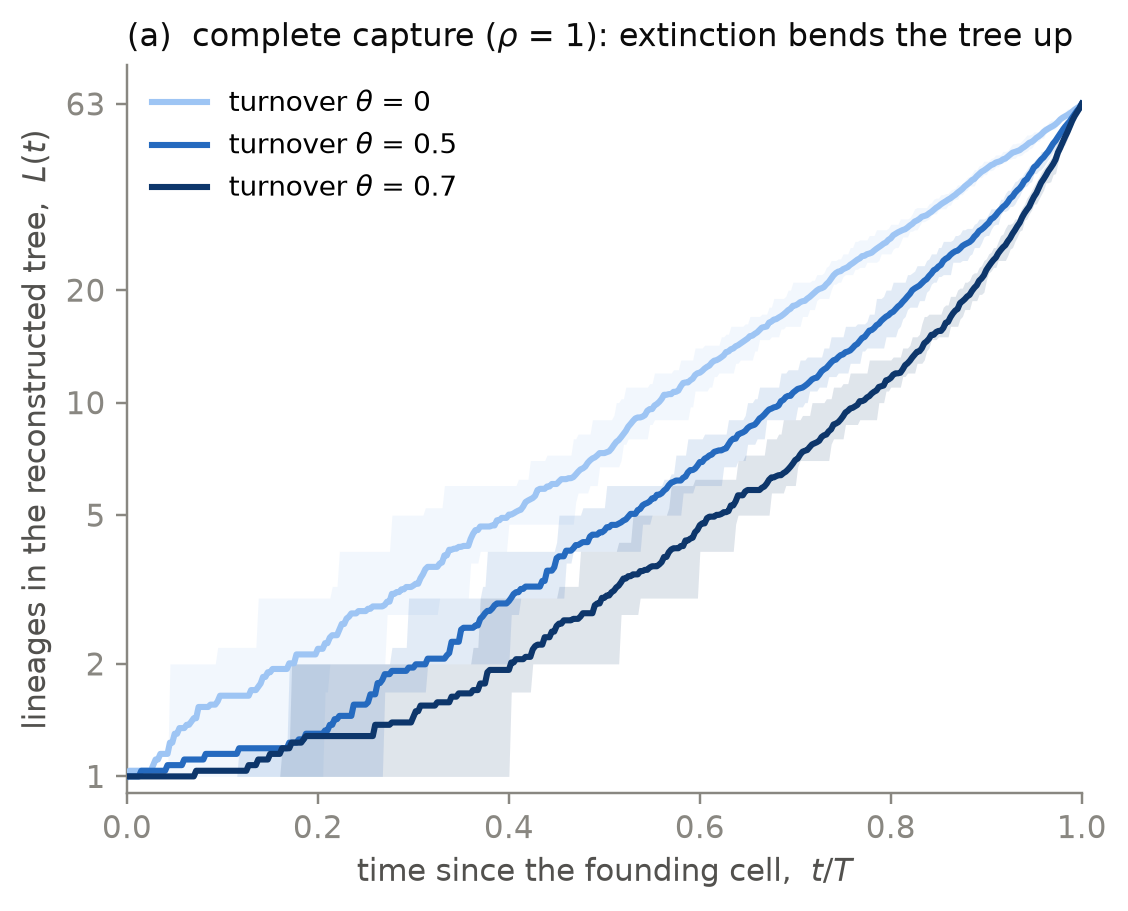
\includegraphics[width=\textwidth]{figS3a_pull}
    \caption{Complete capture.}\label{fig:S3a}
  \end{subfigure}\hfill
  \begin{subfigure}[t]{0.49\textwidth}
    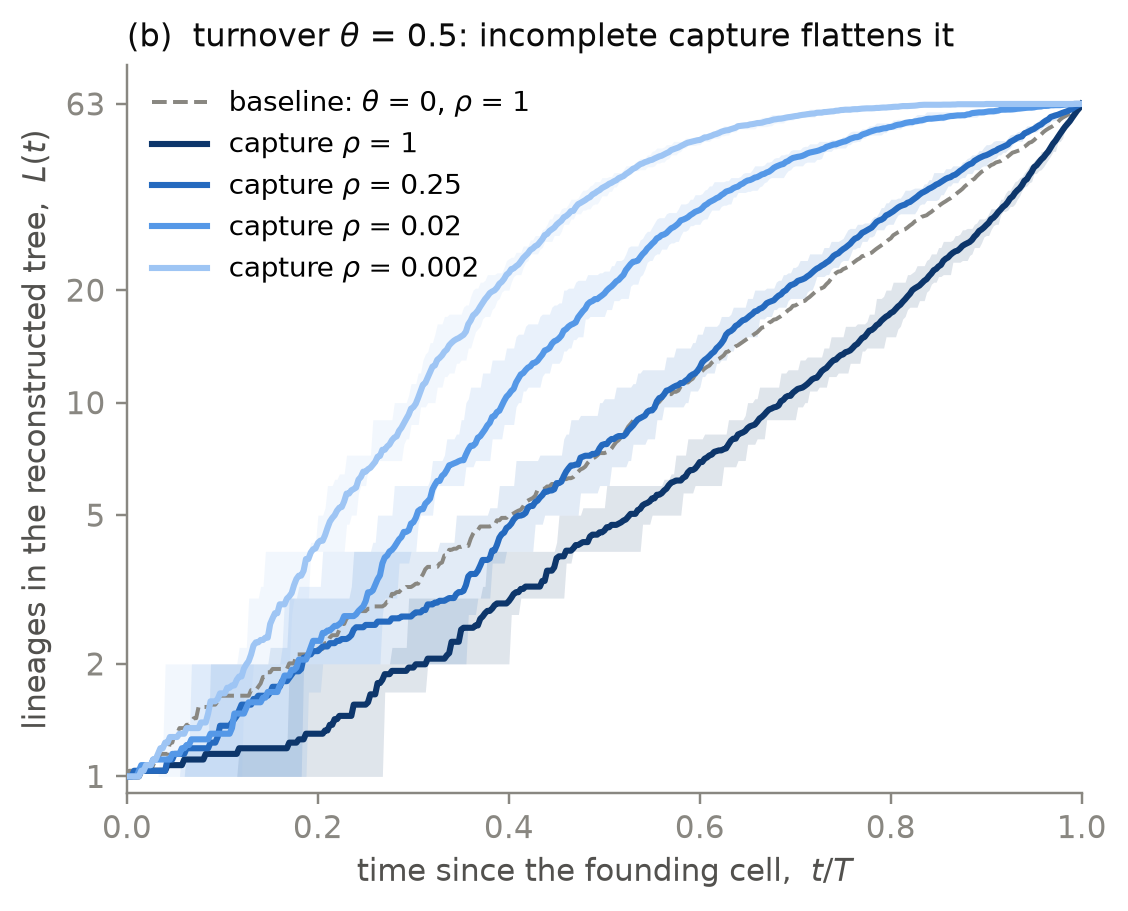
\includegraphics[width=\textwidth]{figS3b_capture}
    \caption{Turnover fixed at $\turn=0.5$.}\label{fig:S3b}
  \end{subfigure}
  \caption{\textbf{The pull of the present, and capture pushing against it.} Lineages in the
  reconstructed tree, log scale, against time since the founding cell. $n=63$, and each curve is
  the mean over 20 trees. Shading marks the middle 50\% of trees.
  \textbf{(a)} With every cell captured ($\capt=1$), zero turnover gives a curve that is close to
  straight: constant visible branching. Turnover bends it upward over the last part of the
  experiment. Over the final tenth of $T$, lineages accumulate at $4.0$ per lineage per unit $T$
  at $\turn=0$, $7.5$ at $\turn=0.5$ and $10.2$ at $\turn=0.7$. That is, $1.9\times$ and
  $2.6\times$ the zero-turnover rate.
  \textbf{(b)} At $\turn=0.5$, lowering capture reverses the bend. Over the final tenth of $T$ the
  rate falls from $7.5$ ($\capt=1$) to $3.2$ ($0.25$), $0.49$ ($0.02$) and $0.008$ ($0.002$). At
  mouse-like capture, essentially no branch point is visible in the last tenth of the experiment,
  and most of the tree's branching sits in its first half. Dashed: the zero-turnover,
  complete-capture baseline.}
  \label{fig:S3ab}
\end{figure}

\begin{figure}[p]
  \centering
  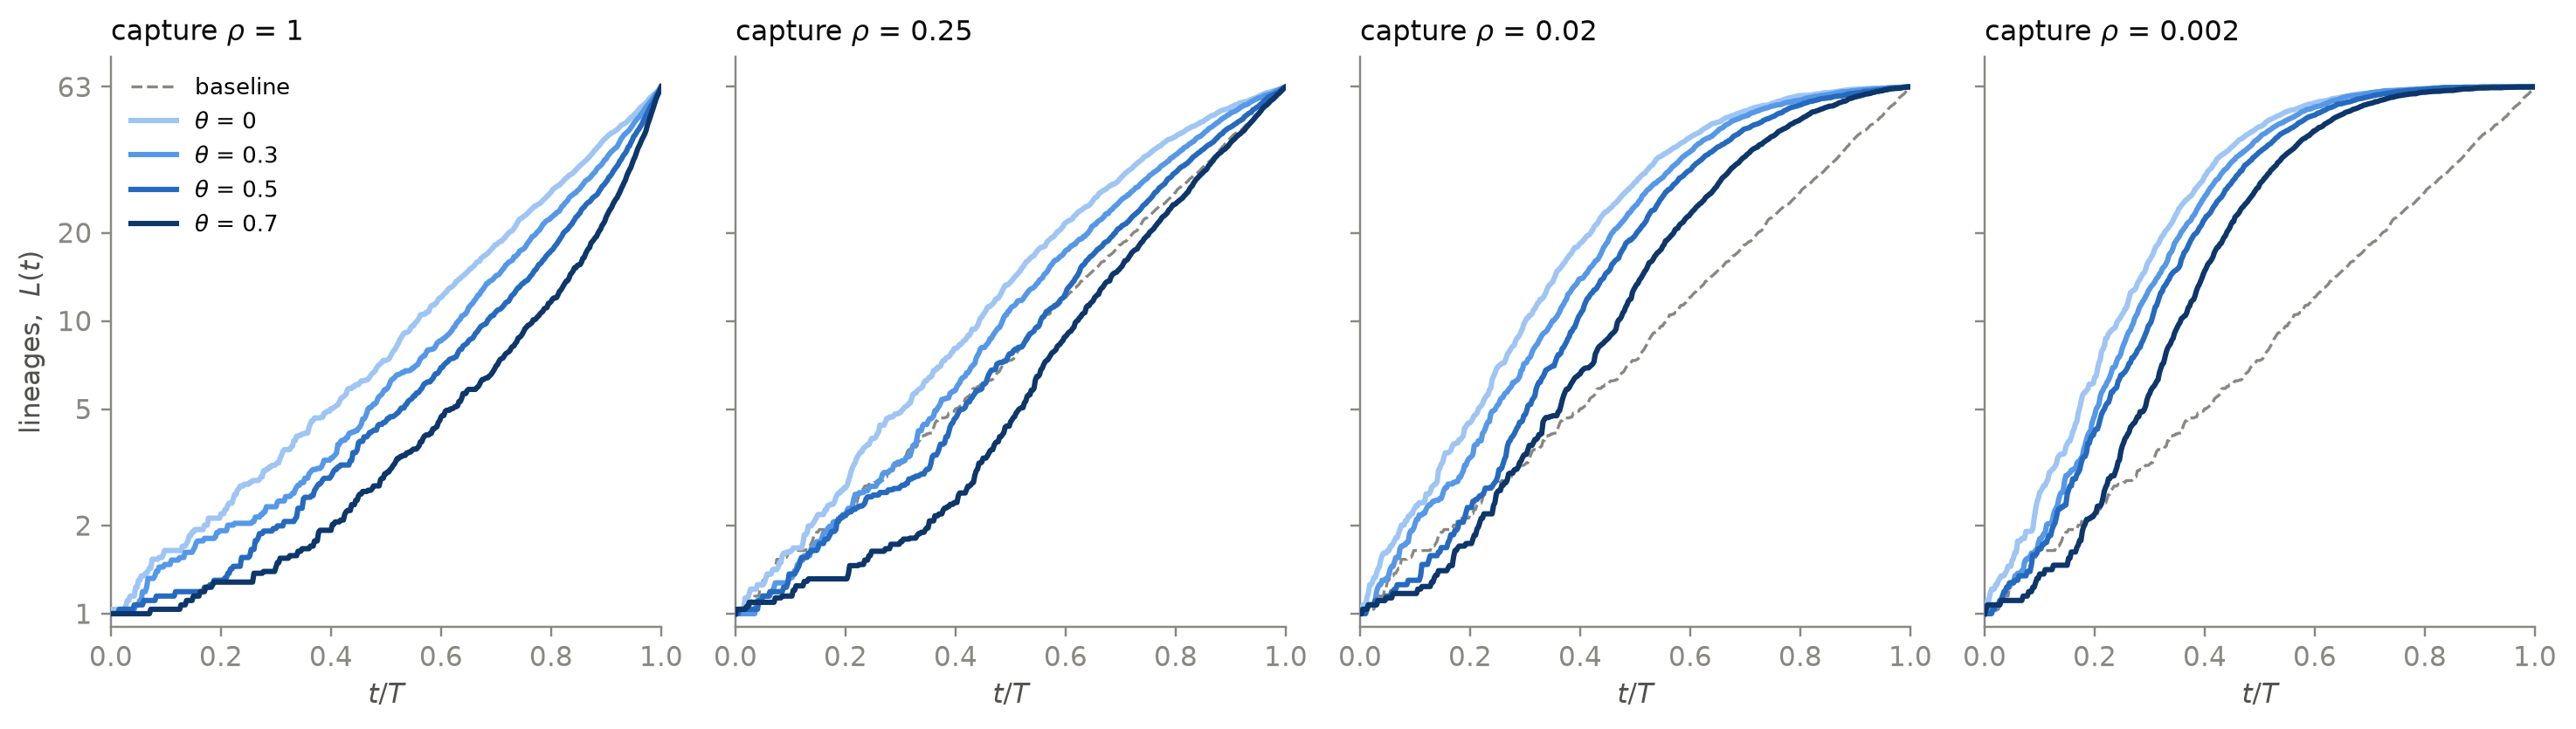
\includegraphics[width=\textwidth]{figS3c_grid}
  \caption{\textbf{Both parameters together.} One panel per capture fraction; lines are turnover
  $\turn\in\{0,0.3,0.5,0.7\}$ (darker is higher). Dashed: the zero-turnover, complete-capture
  baseline, the same in every panel. $n=63$, 20 trees per line, no bands (see Fig.~\ref{fig:S3ab}
  for their width).
  \emph{How turnover shows changes with capture.} At $\capt=1$ it changes the curve's
  \emph{shape}: higher $\turn$ bends it up near harvest. At $\capt=0.002$ the curves have the same
  saturating shape and higher $\turn$ \emph{shifts} them later, by roughly $0.05$--$0.1\,T$.
  Raising $\capt$ also shifts the curve later (Fig.~\ref{fig:S3b}), so at low capture a higher
  turnover and a higher capture fraction move the tree in the same direction.}
  \label{fig:S3c}
\end{figure}

\subsection{Why it matters}

\begin{enumerate}
  \item \textbf{Turnover is invisible in a tree's shape and visible only in its timing.} Given $n$,
        the branching \emph{pattern} of the reconstructed tree does not depend on $\bdrate$,
        $\dthrate$ or $\capt$ (\S\ref{sec:shape}). The bends in Fig.~\ref{fig:S3ab} are therefore
        the only place in the tree where cell death leaves a trace. For a lineage recorder, timing
        is read from edit depths, so any inference of turnover depends on the editing layer
        resolving \emph{when} branch points happened.
  \item \textbf{Capture pushes the opposite way, so an unknown capture fraction can hide or mimic
        turnover.} In Fig.~\ref{fig:S3c}, at low capture, raising $\turn$ and raising $\capt$
        both shift the curve later. For the mouse arms, where $\capt$ is unknown, the tree alone
        may not separate the two (tested formally in neither direction yet). This is the case for
        asking for a total viable cell count per organ at harvest: it pins $\capt$, and with it the
        interpretation of every timing feature of the tree.
  \item \textbf{Where the branching information sits depends on capture.} At complete or high
        capture, the visible branching, and the turnover signal, is concentrated near the harvest.
        At mouse-like capture it moves into the first half of the experiment. That decides when a
        recorder most needs to be writing edits, which is the design question.
\end{enumerate}

\end{document}
